\chapter{\label{chap:development}Desenvolvimento}

O objetivo desse capítulo é apresentar detalhes da implementação, baseados na
modelagem apresentada no Capítulo \ref{chap:modeling}. Na Seção
\ref{section:project-details} apresentamos a arquitetura do projeto, mostrando
como os componentes se relacionam de forma a possibilitar a execução dos
\textit{bots}. Na Seção \ref{section:modifications} apresentamos as
modificações que realizamos no projeto original e os porquês dessas
modificações. Na Seção \ref{section:neat-details} apresentamos detalhes da
implementação do algoritmo \textit{NEAT}. Na Seção \ref{section:analytics}
apresentamos como coletamos e analisamos os dados de nossas execuções.

\section{\label{section:project-details}Detalhamento do Projeto}
O primeiro passo para dar início ao desenvolvimento deste projeto é obter uma
cópia do projeto \textit{SpelunkBots}, hospedada no \textit{website} de
versionamento de código
\textit{GitHub}\footnote{https://github.com/GET-TUDA-CHOPPA/SpelunkBots}. O
\textit{framework} conta com o código modificado do \textit{Spelunky} e uma
distribuição do \textit{GameMaker Pro 8.0}, utilizada para compilar e gerar o
arquivo executável do jogo.

Conforme detalhado na seção \ref{section:spelunkbots}, o \textit{SpelunkBots}
disponibiliza duas opções de linguagem de programação para realizar o
desenvolvimento dos \textit{bots}: \textit{GML} ou C++. Portanto, a próxima
etapa do projeto é definir a linguagem de programação que vamos utilizar. Para
este projeto, escolhemos a linguagem de programação \textbf{C++}, tendo em vista
que o desenvolvimento utilizando a linguagem \textit{GML} é extremamente
limitado. Além disso, é possível encontrar na Internet algumas bibliotecas em
C++ que implementam a técnica
\textit{NEAT}\footnote{http://nn.cs.utexas.edu/?neat-c}. O uso de uma biblioteca
salva tempo de desenvolvimento e permite que o foco do trabalho seja somente no
desenvolvimento dos \textit{bots}, e não na arquitetura necessária para tal.

Sabendo que a técnica \textit{NEAT} requer que o \textit{bot} receba treinamento
através de diversas simulações do jogo, optamos pelo uso de um servidor
dedicado, pois este processo pode ser demorado e realizá-lo em uma máquina
doméstica -- que está muito mais sujeita a ser desligada acidentalmente ou
intencionalmente -- seria arriscado. O servidor em questão utiliza um sistema
operacional baseado em \textit{Linux}.  Contudo, \textit{Spelunky} foi
desenvolvido utilizando uma versão muito antiga do \textit{GameMaker} e a
compilação do código externo do \textit{SpelunkBots} ocorre através de um
projeto em \textit{Visual Studio}.  Estas ferramentas só podem ser executadas no
sistema operacional \textit{Windows}. Como nosso servidor é baseado em
\textit{Linux}, é necessário realizar algumas adaptações no processo de
compilação e execução. Assim, utilizamos os \textit{softwares}
\textit{MinGW}\footnote{http://www.mingw.org} e
\textit{Wine}\footnote{https://winehq.org}, que nos permitiram, respectivamente,
realizar uma compilação cruzada\footnote{Um compilador cruzado, ou
	\textit{cross-compiler}, é uma ferramenta de compilação capaz de produzir
código executável em uma plataforma diferente da qual o compilador está sendo
executado.} do código C++ para da plataforma \textit{Linux} para a plataforma
\textit{Windows}, gerando uma \textit{DLL}, e executar programas da plataforma
\textit{Windows} dentro do sistema operacional \textit{Linux}.

O próximo passo foi escolher a biblioteca de inteligência artificial da técnica
\textit{NEAT} e incluí-la no processo de compilação da \textit{DLL},
integrando-a ao projeto \textit{SpelunkBots}. Ao concluir este passo, as
configurações iniciais do projeto foram finalizadas e iniciamos o processo de
modelagem e desenvolvimento dos \textit{bots}. O diagrama
\ref{fig:project-diagram} ilustra a relação entre os elementos de configuração
do projeto.

\begin{figure}[h]
\centering
\begin{tikzpicture}
    \tikzstyle{every node}=[font=\footnotesize, text centered]
    \node (gmm) at (0, 0)  {Game Maker};
    \node (spl) at (0, -2) {Spelunky};
    \node[draw] (spb) at (0, -4) {SpelunkBots};

    \node[text width=4cm] (conf) at (5, 0)  {Configurações \\(escolha do bot e parâmetros de nível)};
    \node (comp) at (5, -4)  {Compilação (MinGW)};

    \node[draw] (neat) at (11, 0) {Biblioteca NEAT};

    \node (dll) at (11, -2) {Solução DLL};

    \node[draw] (bots) at (11, -4) {Código dos \textit{bots}};

    \node at (0, -6) (wine) {Emulação (WineHQ)};

    \node at (5, -6) (linux) {Servidor Linux};

    \node[draw, inner sep=.25cm, fit={(gmm) (spl) (spb)}] (g2) {};
    \node[draw, fit={(spl) (spb)}] {};

    \node[draw, fit={(dll) (bots)}] (g1) {};

    \draw[->, >=latex] (neat.south) -- (g1.north);

    \draw[->, >=latex] (g1.west) -- (comp.east);
    \draw[->, >=latex] (comp.west) -- (spb.east);

    \draw[->, >=latex, in=0, out=200] (conf.west) to (spb.east);

    \draw[->, >=latex] (g2.south) -- (wine.north);
    \draw[->, >=latex] (wine.east) -- (linux.west);
\end{tikzpicture}
\caption {Diagrama do projeto explicando a relação entre os componentes
necessários para o desenvolvimento dos \textit{bots}.
}
\label{fig:project-diagram}
\end{figure}

O \textit{framework} \textit{SpelunkBots} provê uma interface comum para o
desenvolvimento dos \textit{bots} em C++, chamada \textbf{\textit{IBot.h}}. Esta
interface é responsável por expor os métodos e variáveis que os \textit{bots}
utilizam para comunicar-se com o jogo. Portanto, qualquer código de \textit{bot}
desenvolvido deverá partir desta interface. Analisando o arquivo \textit{IBot.h}
é possível perceber que a interface obriga o desenvolvedor a implementar
\textbf{pelo menos} o método \textbf{\textit{Update}}, chamado em todas as
etapas de execução do \textit{bot} para receber informações e enviar comandos ao
jogo. Existem dois outros métodos que podem ser úteis ao desenvolvedor, mas que
não possuem obrigatoriedade de implementação: o \textbf{\textit{Reset}} e o
\textbf{\textit{NewLevel}}. O método \textit{Reset} é chamado no início de todas
as etapas de execução do \textit{bot} para reiniciar suas variáveis de controle.
Este método possui uma implementação padrão que reinicia apenas as variáveis
essenciais (esquerda, direita, pular e atacar). O método \textit{NewLevel} é
chamado toda vez que o \textit{bot} entra em um novo nível, e pode ser usado
para descartar informações do nível anterior sem que seja necessário reiniciar
todas as variáveis do \textit{bot}. Em sua implementação padrão, não executa
nada.

Uma implementação mínima de um \textit{bot} utilizando a interface
\textit{IBot.h} necessitaria, portanto, de dois arquivos: um arquivo
\textit{header}, que conterá as declarações dos métodos e variáveis a serem
utilizadas -- demonstrado no Algoritmo \ref{alg:project-example-bot-header} --,
e um arquivo de implementação -- demonstrado no Algoritmo
\ref{alg:project-example-bot-impl} --, que conterá a implementação das funções
descritas no arquivo \textit{header}.

\section{\label{section:modifications}Modificações do Código Original}

O código original do jogo conta com algumas características e limitações que
dificultavam o desenvolvimento desse trabalho. Contudo, temos acesso ao
código-fonte e somos capazes de modificá-lo. Assim, esta seção detalha as
modificações que fizemos, de forma a facilitar ou viabilizar o desenvolvimento.

\subsection{\textit{Scripts} de Compilação}

A escolha da linguagem \textit{C++} para a criação dos \textit{bots} requer a
compilação e geração de uma \textit{DLL} para que, posteriormente o
\textit{SpelunkBots} utilize-a. Este processo é feito em várias etapas.
Primeiro, compilamos as bibliotecas que utilizamos. Em seguida, compilamos o
código dos \textit{bots} e geramos a \textit{DLL}. Por fim, movemos a
\textit{DLL} para o local onde o \textit{SpelunkBots} será executado.

É necessário executar com sucesso todas as etapas de compilação para viabilizar
o desenvolvimento dos \textit{bots}. De forma a automatizar esse processo,
criamos um \textit{script} -- utilizando \textit{shell script} -- responsável
pelo processo de compilação e movimentação de arquivos.

\subsection{Pular Cena Inicial do Jogo}

O \textit{Spelunky} conta com uma cena inicial onde o jogador se desloca da
superfície para dentro de uma caverna. Esta caverna serve como menu principal do
jogo permitindo que o jogador escolhe entre fazer o tutorial do jogo, inciar sua
aventura, ver as maiores pontuações, entre outros. A Figura
\ref{fig:spelunky-introduction} apresenta a cena inicial e a caverna de menu
principal.

\begin{figure}[H]
\centering
	\begin{subfigure}[b]{0.4\textwidth}
		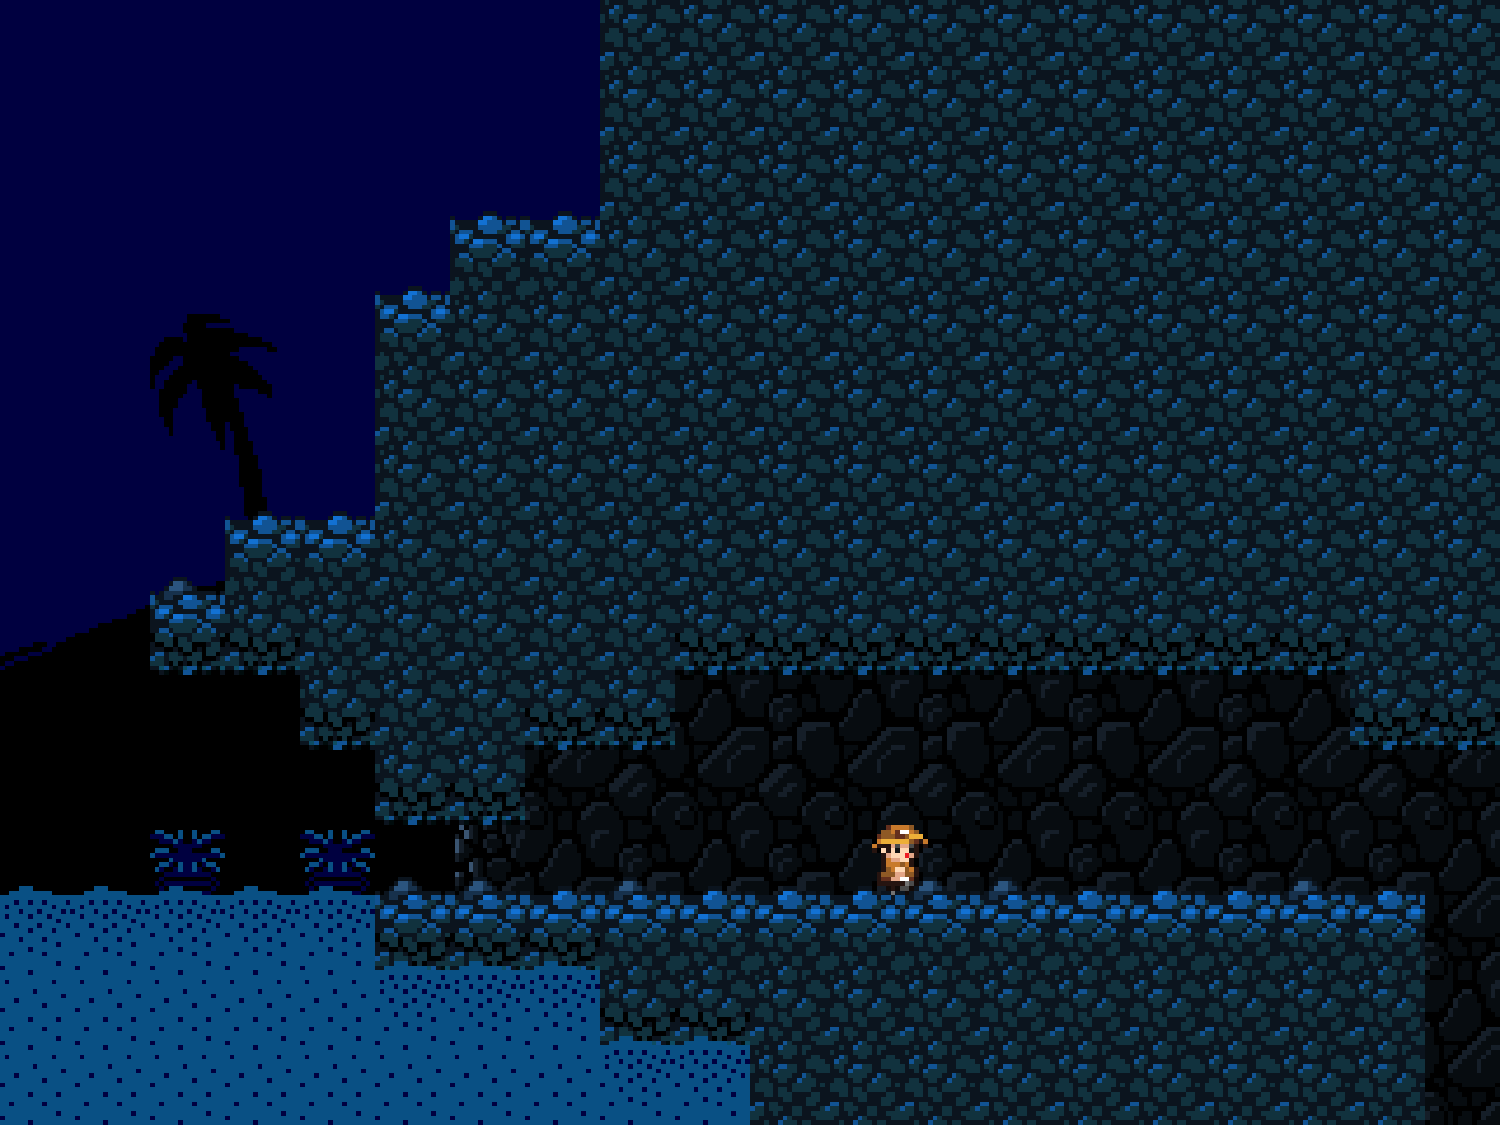
\includegraphics[width=\textwidth]{fig/spelunky-intro-screen.pdf}
		\caption{Entrada para a caverna inicial.}
		\label{fig:spelunky-intro-screen}
	\end{subfigure}
	\begin{subfigure}[b]{0.4\textwidth}
		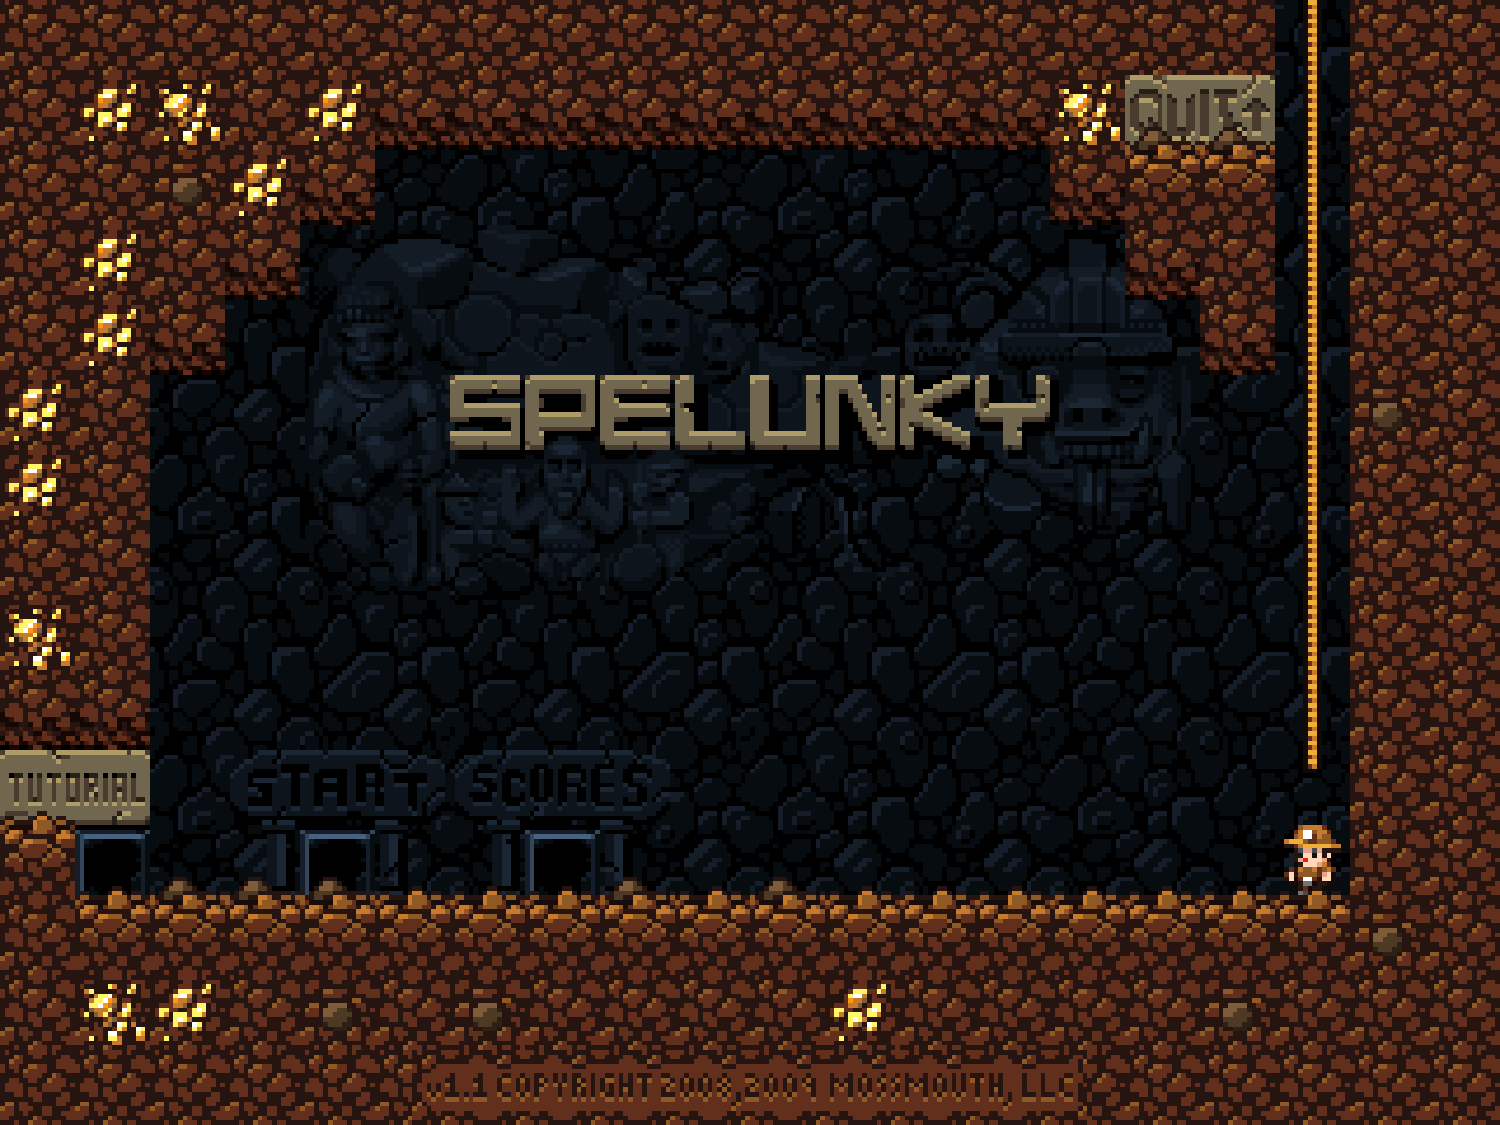
\includegraphics[width=\textwidth]{fig/spelunky-initial-screen.pdf}
		\caption{Caverna de escolha.}
		\label{fig:spelunky-initial-screen}
	\end{subfigure}

    \caption{Cena de introdução do jogo, onde o jogador se desloca da
    superfície para uma caverna com opções de interação.}
	\label{fig:spelunky-introduction}
\end{figure}

Estas cenas são apenas uma forma de introdução ao jogo, não contribuíndo para a
geração de resultados de execução. Logo, não necessitamos delas. Nossos
\textit{bots} devem ser levados diretamente até a opção de iniciar o jogo nos
mapas customizados que geramos.  Assim, utilizamos \textit{GameMaker} para
remover essas cenas. Portanto, ao executar o jogo, o \textit{bot} é levado
diretamente ao nível escolhido, executando imediatamante.

\subsection{Interrupção da Execução de Agentes não Promissores}

Devido às limitações apresentadas anteriormente na seção
\ref{section:spelunkbots-limitations}, é muito importante conseguirmos definir o
momento em que algum \textit{bot} esteja em um estado não promissor -- gastanto
tempo de execução --. Isso permite que interrompamos a execução, acelerando o
processo de treinamento.  Para isso, definimos dois critérios que nos concedem a
capacidade de identificar o momento em que um \textit{bot} está ocioso:

\begin{description}
	\item [Tempo parado] em alguns casos, o \textit{bot} pode escolher ficar
		parado. Porém, caso ele fique ocioso por muito tempo, é muito provável
		que nada de diferente ocorrerá até o fim da execução, dado que não
		existem elementos dinâmicos em nossos testes. Assim, quando
		identificamos que o \textit{bot} está parado há mais de \textbf{3
		segundos}, interrompemos sua execução, sinalizando sua ociosidade para
		aa função de aptidão.

	\item [Estados repetidos] o único elemento dinâmico em nossos testes é a
		posição do jogador no mapa. Portanto, podemos considerar que o estado do
		jogo depende das coordenadas do jogador. Caso o agente visite o mesmo
		estado mais de \textbf{10 vezes}, é possível identificar que ele está
		repetindo excessivamente suas ações e, possivelmente, não sairá de uma
		mesma região, não encontrando a porta de saída. Se este for o caso,
		interrompemos sua execução, sinalizando sua repetição de estados para a
		função de aptidão.
\end{description}

Com estes critérios de interrupção definidos, é necessário que tenhamos uma
forma de parar a execução do agente caso um dos cenários descritos acima ocorra.
Assim, implementamos uma função de \textbf{verificação de ociosidade} e uma
variável \textit{booleana} de suicídio no código do \textit{bot}. A cada ciclo
de execução do jogo, averiguamos se o \textit{bot} está parado e, caso esteja,
incrementamos um contador de tempo (este contador é zerado caso haja
movimentação). Após, incrementamos o contador que indica o número de vezes que o
\textit{bot} visitou a posição em que se encontra atualmente. Caso ele esteja
parado pelo determinado número de segundos ou tenha visitado o mesmo estado pelo
determinado número de vezes, sabemos que esse é um estado não promissor. Então,
ativamos a variável de suicídio cujo propósito é zerar o número de pontos de
vida do jogador, fazendo com que o \textit{bot} reinicie sua execução.

\subsection{Arquivo de Inicialização}

O processo de escolha das configurações para a execução do jogo requer
experimentação. É necessário combinar diferentes parâmetros e avaliar sua
execução, escolhendo então os parâmetros que produzem os melhores resultados.
No caso do \textit{SpelunkBots}, esta escolha está ligada diretamente à edição
do código do jogo no \textit{Game Maker}. Sempre que desejamos editar um
parâmetro de execução, abrimos o \textit{software}, realizamos a edição dos
valores, salvamos uma nova versão do jogo e então o executamos. Esse processo é
manual e custoso, dificultando a escolha dos melhores parâmetros para execução.  

Dessa forma, alteramos o código do \textit{SpelunkBots} para permitir a leitura
de um arquivo de inicialização
(\textit{.INI})\footnote{https://docs.yoyogames.com/source/dadiospice/002\_reference/file\%20handling/ini\%20files/index.html}.
Assim, podemos alterar os valores dos parâmetros de execução sem abrir o
\textit{GameMaker} para recompilar o código e gerar um novo arquivo executável.
Um arquivo \textit{.INI} é dividido em \textbf{seções} e cada seção possui
\textbf{pares} de chave para valor associado.

O Algoritmo \ref{alg:ini-file} apresenta um exemplo de arquivo de inicialização.
Utilizamos quatro seções distintas para diferenciar o propósito dos pares de
valor. \textit{\textbf{[Bot]}} representa as informações sobre o \textit{bot}
escolhido na execução. A entrada \textit{bot\_is\_cpp}, quando com o valor
\textbf{1}, indica que se trata de um \textit{bot} que foi escrito em
\textit{C++}, já a entrada \textit{bot\_cpp\_num} idica qual \textit{bot} será
executado.  A seção \textit{\textbf{[Test]}} informa dados relativos ao teste
que será realizado. O tipo de mapa é informado pela entrada \textit{test\_type}.
O parâmetro \textit{test\_rank} indica ao \textit{SpelunkBots} como classificar
a execução dos \textit{bots}. Podemos controlar o número \textbf{máximo} de
execuções pelo valor de \textit{test\_num}. Também é possível limitar o tempo de
vida de um \textit{bot} pelo parâmetro \textit{test\_time}, que é indicado em
segundos.  É possível especificar os níveis que queremos utilizar para testar os
agentes através da seção \textit{\textbf{[Levels]}}. Primeiro, indicamos a
quantidade de níveis pelo valor de \textit{level\_num}. Após, para cada nível,
indicamos o seu nome em uma propriedade específica. No caso do primeiro, usamos
a propriedade \textit{level0}, para o segundo, \textit{level1}, e assim para
todos eles.  Por fim, temos a seção \textit{\textbf{[FAMW]}}, que parametriza a
exibição de informações de depuração durante a execução do jogo.  O valor de
\textit{vision\_debug} indica se deverá ser exibida na tela uma janela da visão
do \textit{bot}, com o tamanho informado por \textit{vision\_size}.

\begin{algorithm}[H]
\lstinputlisting[style=customC++]{code/spelunkbots.ini}
	\caption[Exemplo de um arquivo de inicialização \textit{.INI}.]
{\label{alg:ini-file}Arquivo de inicialização de exemplo.}
\end{algorithm}

\subsection{\label{sub:virtual-display}Execução com Display Virtual}

Como vimos anteriormente, na seção \ref{section:spelunkbots-limitations}, não é
possível executar o jogo sem janela gráfica. Isto é um problema, pois o servidor
\textit{Linux} que utilizamos para a execução dos testes não possui nenhuma
interface gráfica.  Porém, é possível superar esta limitação através da
utilização de um \textit{display} virtual, onde simulamos uma interface gráfica
semelhante a uma real. Nesse caso, utilizamos o \textit{software}
\textit{XVFB}\footnote{https://www.x.org/archive/X11R7.6/doc/man/man1/Xvfb.1.xhtml},
criando então uma interface gráfica que recebe a execução do jogo. O uso de uma
interface gráfica virtual também nos permitiu realizar conexões remotas para o
servidor, concedendo-nos a capacidade de acompanhar o processo de treinamento em
tempo real.

\subsection{\label{sub:spelunkbots-gui}Interface de Acompanhamento do
SpelunkBots}

O \textit{SpelunkBots} conta com uma interface de acompanhamento da execução do
jogo. Além de possibilitar ver o personagem explorando a caverna, ela também
mostra alguns controles específicos do \textit{SpelunkyBots}, tais como os
botões que o jogador está apertando, além de algumas informações de direção.

Embora essa interface contenha muitas informações, muitas delas não são
relevantes no nosso caso. Além disso, implementamos alguns controles para o
jogo -- tal como o tempo máximo de execução -- que são interessantes de
acompanharmos. Portanto, modificamos essa tela de acompanhamento, deixando
apenas as informações que consideramos relevantes. Nesse caso, a direção para
onde o jogador está se movimentando e se ele está apertando o botão de pular.
Além disso, também queremos saber o tempo restante de execução. Assim, criamos
um contador que inicia com o tempo máximo estipulado vai sendo decrementado ao
longo do tempo. Também adicionamos um quadrado vermelho em volta do jogador,
indicando o campo de visão dele. A Figura \ref{fig:spelunkbots-gui} compara a
interface antes e depois das modificações.

\begin{figure}[H]
\centering
	\begin{subfigure}[b]{0.4\textwidth}
		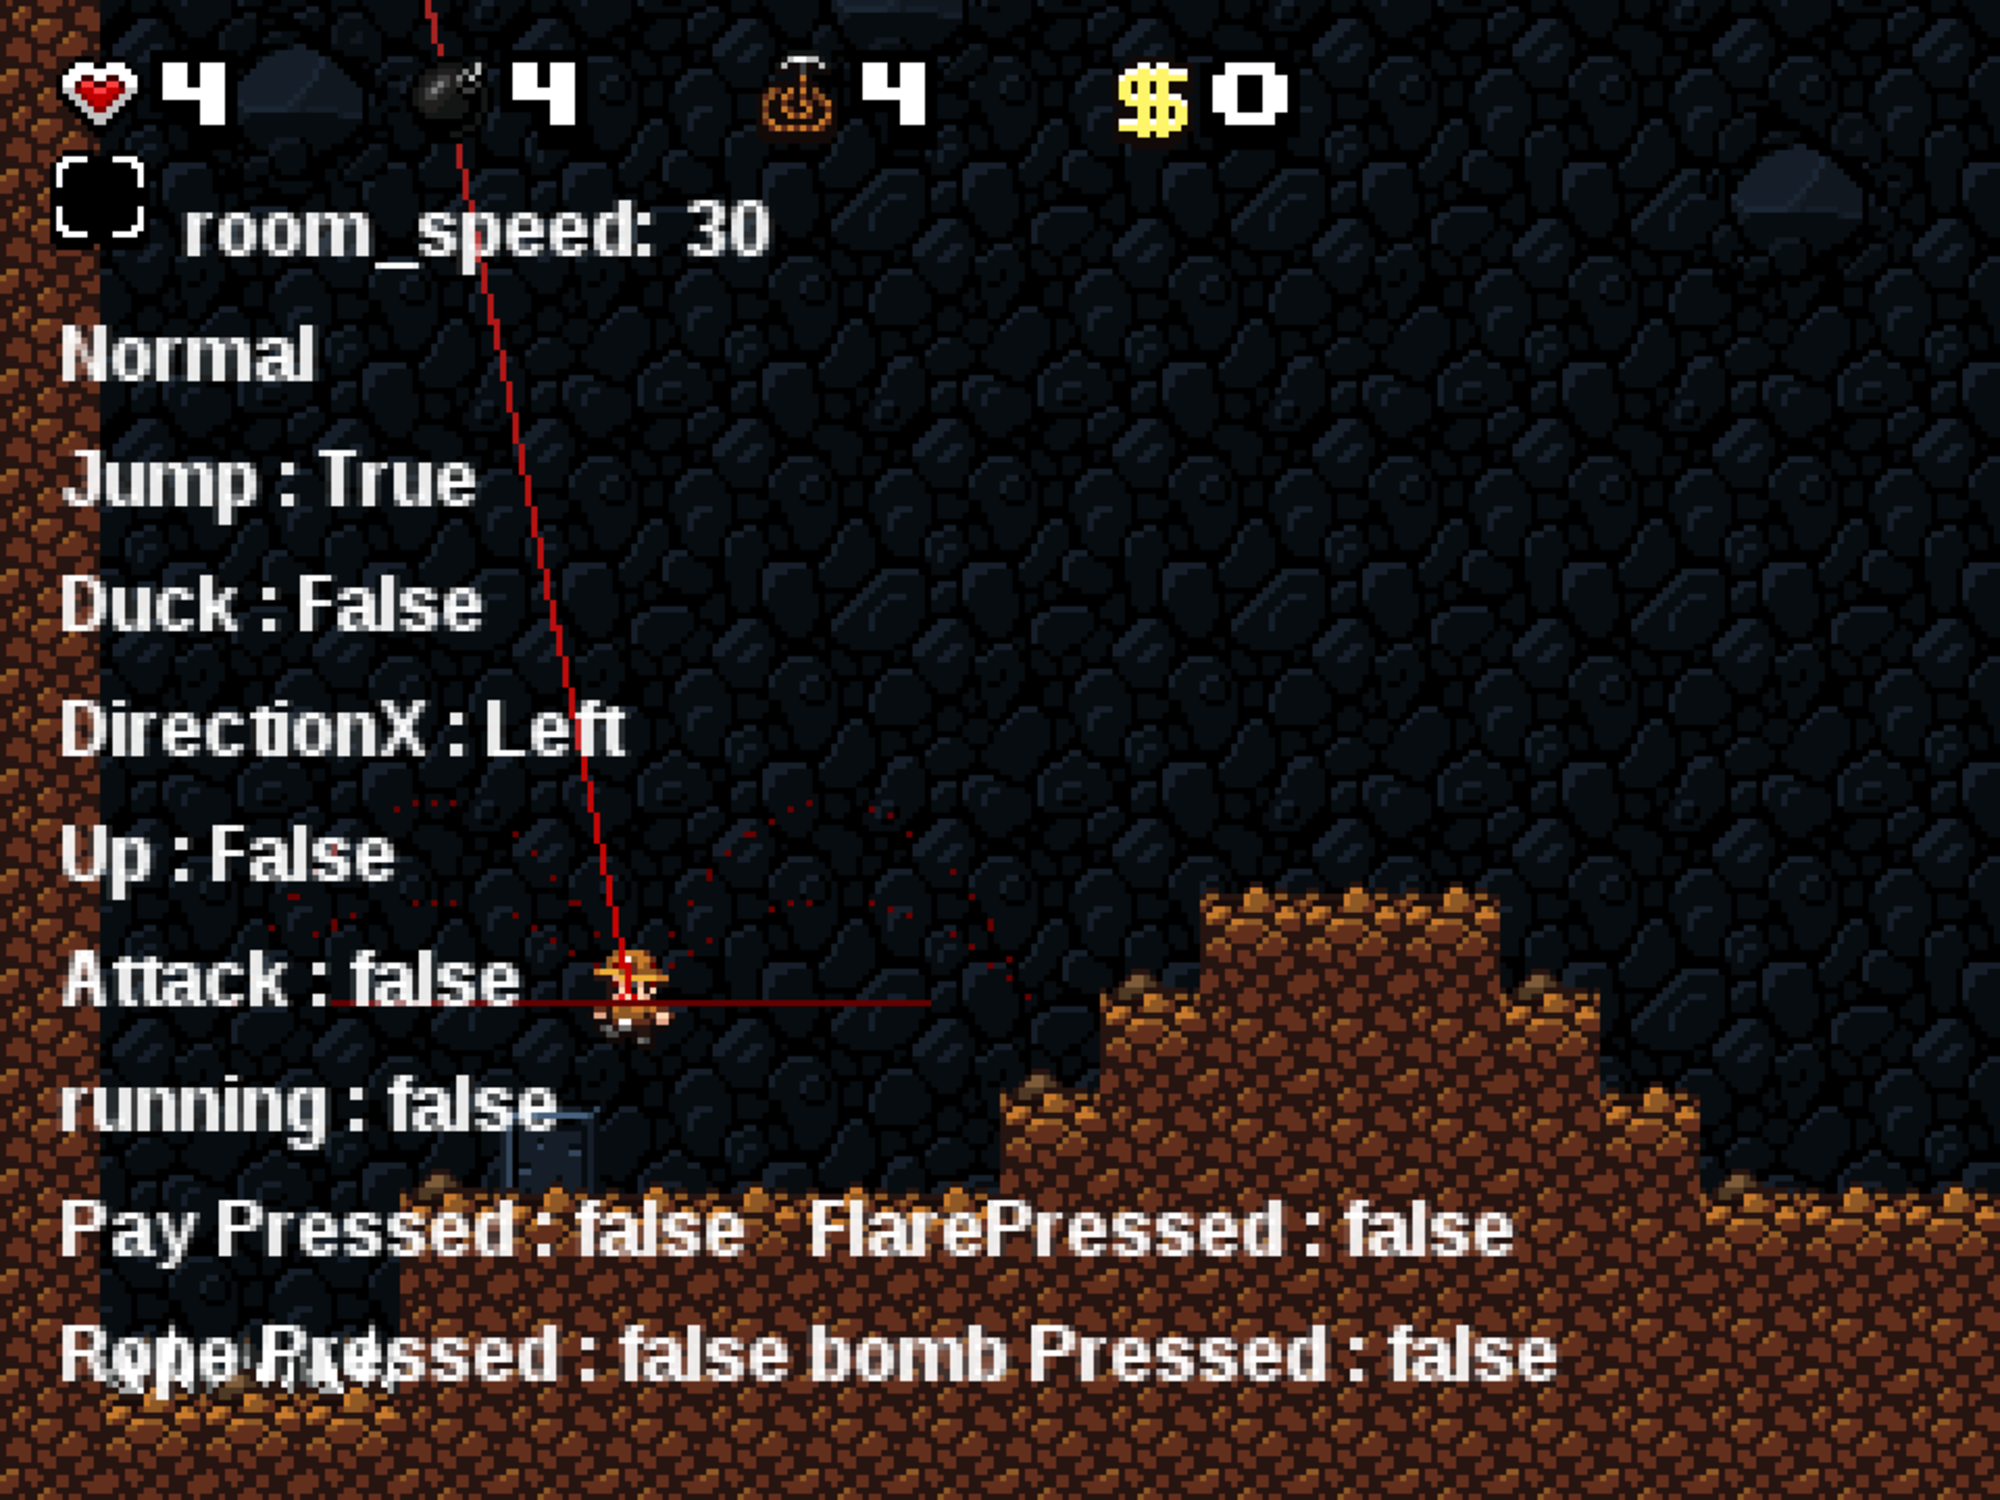
\includegraphics[width=\textwidth]{fig/spelunkbots-gui-before.pdf}
        \caption{Interface do \textit{SpelunkBots} antes das modificações realizadas.}
		\label{fig:spelunkbots-gui-before}
	\end{subfigure}
	\begin{subfigure}[b]{0.4\textwidth}
		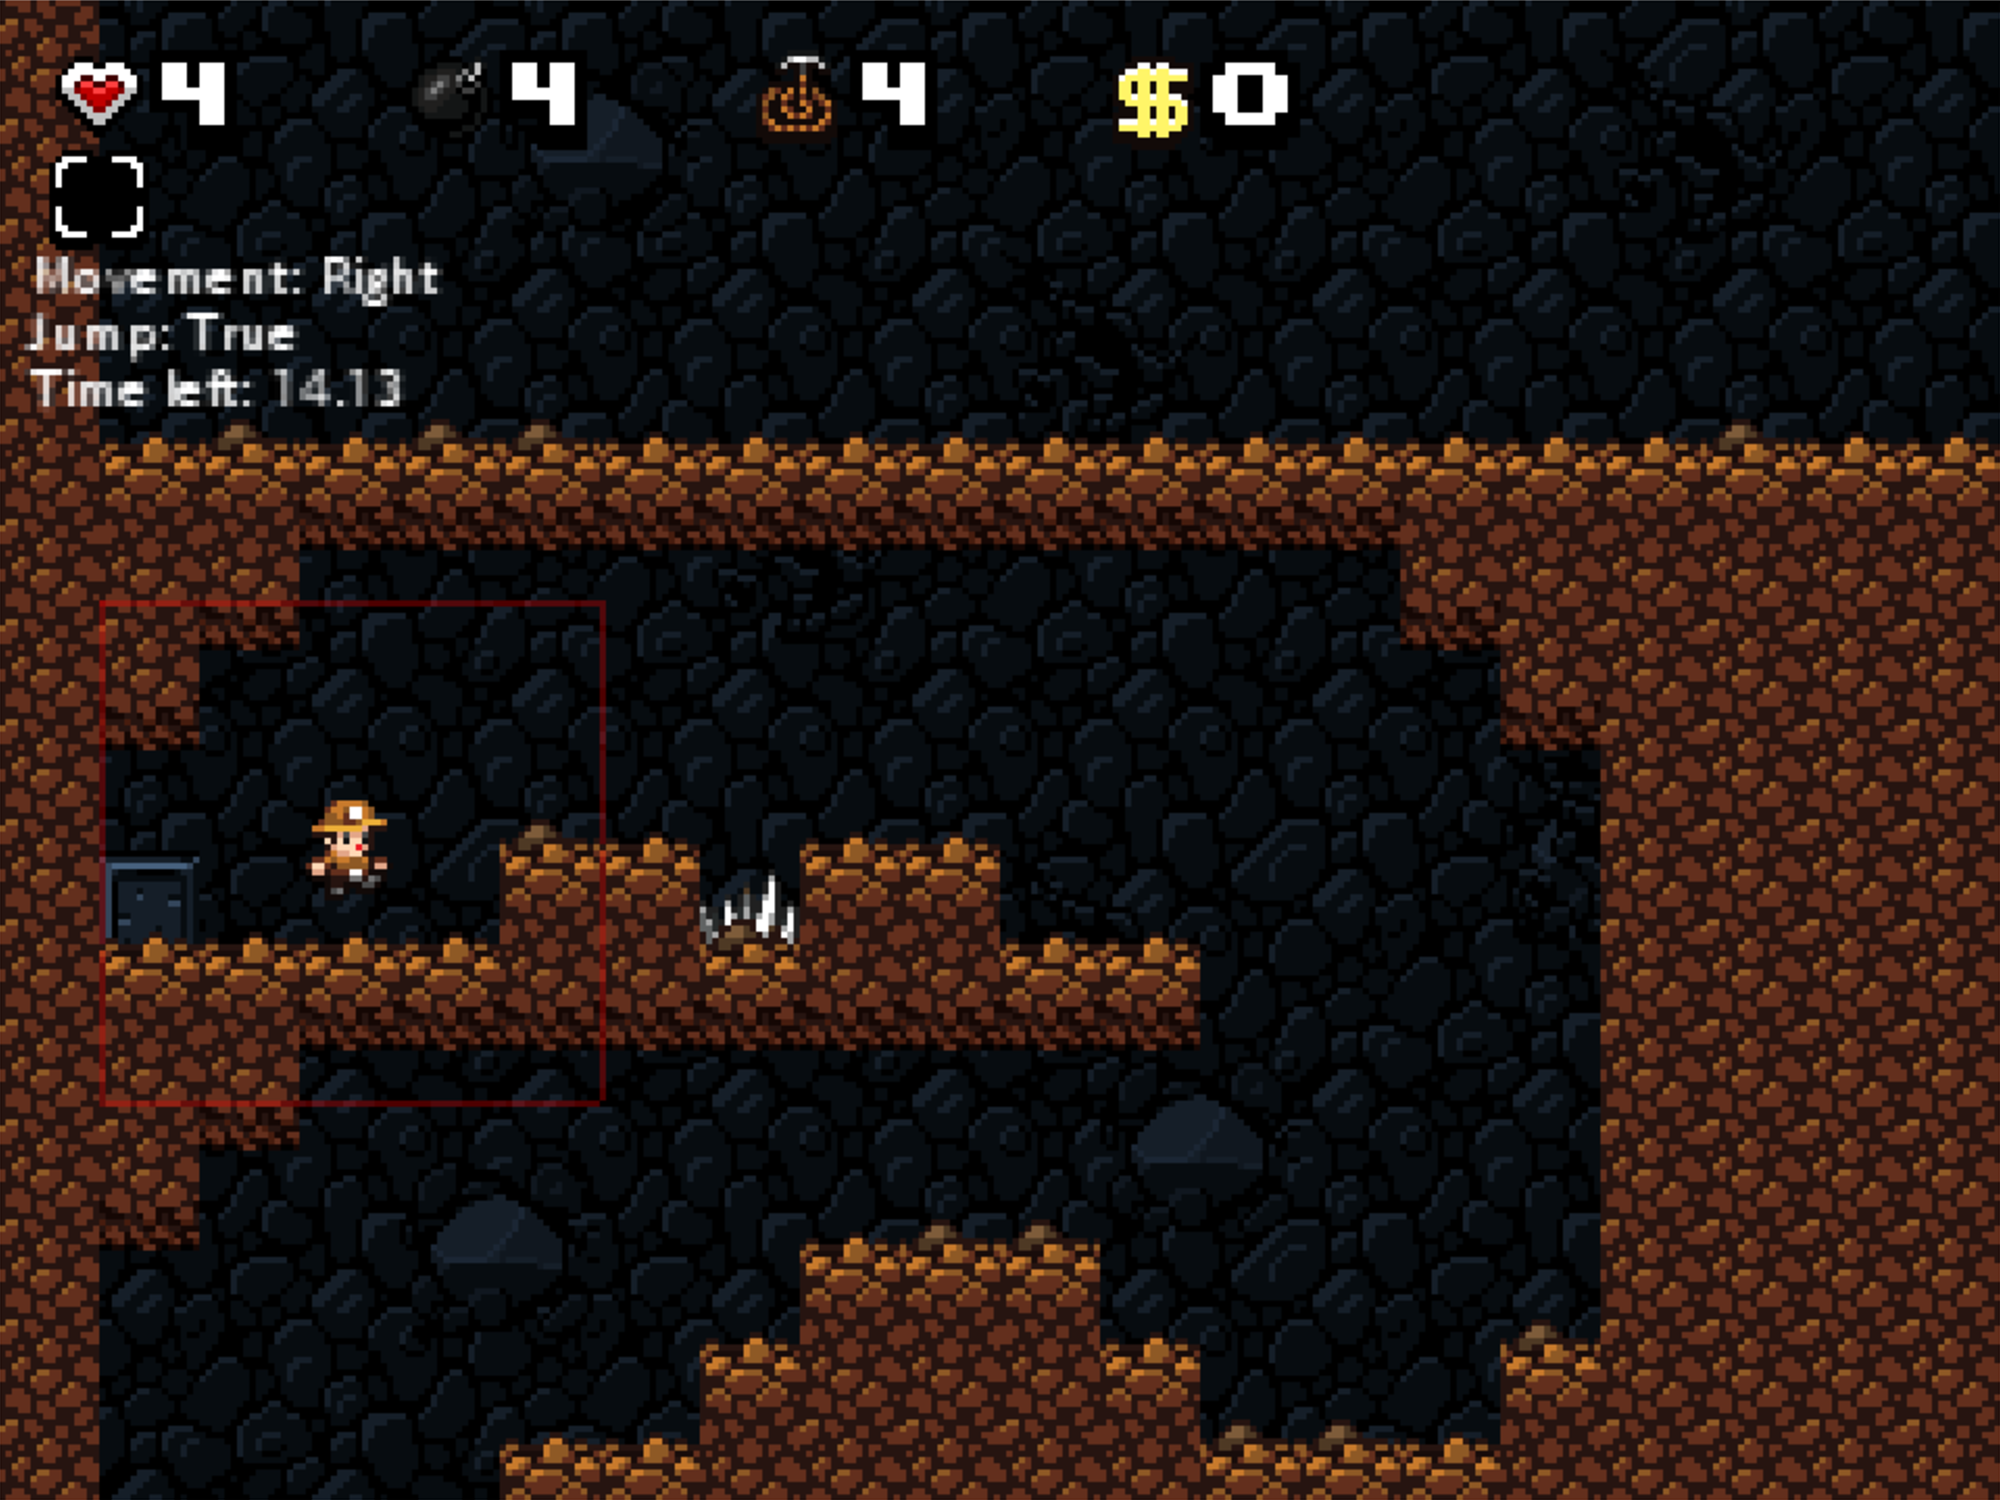
\includegraphics[width=\textwidth]{fig/spelunkbots-gui-after.pdf}
        \caption{Interface do \textit{SpelunkBots} após as modificações realizadas.}
		\label{fig:spelunkbots-gui-after}
	\end{subfigure}

    \caption{Comparação entre a interface do \textit{SpelunkBots} antes e
    depois das modificações realizadas.}
	\label{fig:spelunkbots-gui}
\end{figure}

\section{\label{section:neat-details}Implementação do NEAT}
Com o objetivo de poupar tempo na parte do desenvolvimento, optamos por utilizar
a biblioteca que implementa o algoritmo \textit{NEAT} disponibilizada pelo autor
da técnica\footnote{http://nn.cs.utexas.edu/?neat-c}. Antes de executar qualquer
treinamento, é necessário entender como configurar os parâmetros de execução da
biblioteca:

\begin{description}
	\item[Valor de Semente]
		A biblioteca utiliza um gerador de números pseudo-aleatórios para
		realizar a decisão de eventos randômicos como, por exemplo, decidir se
		vai mutacionar ou cruzar organismos, selecionar pais para cruzamento,
		entre outros. Portanto, é necessário abastecer este gerador com um valor
		de semente.

	\item[Configurações de Mutação]
		O desenvolvedor deve fornecer um arquivo de texto para a biblioteca com
		as configurações de mutação que deseja utilizar. O Algoritmo
		\ref{alg:neat-parameters-example}, localizado dentro do Apêndice
		\ref{appendix:neat-configs}, possui um exemplo de arquivo de
		configuração de valores de mutação.

	\item[Rede Neural Inicial]
		Outro requisito da biblioteca é que o desenvolvedor forneça um arquivo
		de texto contendo uma configuração de rede neural artificial. A
		biblioteca irá se basear neste arquivo para criar as redes neurais dos
		organismos pertencentes à população inicial. O Algoritmo
		\ref{alg:neat-network-example}, localizado dentro do Apêndice
		\ref{appendix:neat-configs}, possui um  exemplo de arquivo de
		configuração de rede neural inicial.
\end{description}

Para tentar garantir a reprodutibilidade de nossos testes, utilizamos a mesma
semente para popular o gerador de números pseudo-aleatórios em todas as
execuções: \textbf{12345}. Com estes parâmetros iniciais, a biblioteca é capaz
de gerar uma população inicial que respeite as estrutura de rede neural inicial
e evoluí-la de acordo com as configurações de mutação desejadas. Como o arquivo
de rede neural inicial é trabalhoso de se elaborar, desenvolvemos um programa em
C++ que gera automaticamente um arquivo de rede inicial dadas as especificações
desejadas\footnote{https://github.com/famw/neat-startgene-generator}.

Simplificando, o laço de execução do programa do agente, depois do carregamento
dos parâmetros de configuração, ocorre da seguinte maneira: primeiro, coletamos
as informações do jogo utilizando o \textit{SpelunkBots}. Em seguida, carregamos
estas informações nas entradas da rede neural do agente. Após, utilizamos a
função de ativação da rede neural para realizar o processamento dos dados.
Então, coletamos os valores dos neurônios da camada de saída da rede e
selecionamos, de acordo com os valores, quais ações o agente deseja executar.
Por fim, enviamos os comandos de ação ao \textit{SpelunkBots}, que executa-os
para nós.


\section{\label{section:analytics}Análise dos Dados}

A biblioteca de \textit{NEAT} escolhida gera uma série de informações dos
organismos ao fim de cada geração, como valor de aptidão, espécie do organismo,
identificação se o organismo foi vencedor ou não, entre outras. Estas
informações são extremamente úteis, pois podemos utilizá-las para realizar uma
análise do desempenho dos agentes, gerando gráficos ou tabelas com compilados de
informações. O Algoritmo \ref{alg:neat-output-example} mostra um exemplo deste
arquivo de texto para uma geração durante o treinamento.

\begin{algorithm}[H]
\lstinputlisting[style=customC++]{code/gen_example.pop}
\caption[Exemplo de arquivo de execução de um \textit{bot}.]
{\label{alg:neat-output-example}Exemplo de arquivo de execução de um
    \textit{bot}.}
\end{algorithm}

Logo, o próximo passo para analisar os dados foi escolher \textbf{o que queremos
analisar}. Decidimos que o mais interessante é analisarmos o \textbf{número de
organismos vencedores ao longo das gerações} e o \textbf{valor da função de
aptidão ao longo das gerações}. Em seguida, escolhemos que ferramenta iríamos
utilizar a fim de gerar visualizações mais intuitivas para estes dados
coletados. Como as nossas comparações são representadas por um valor -- ou o
número de vencedores, ou um valor de aptidão -- em função de um número gerações,
utilizamos uma \textbf{representação gráfica} que permite analisar esses
valores. Portanto, escolhemos o
\textit{gnuplot}\footnote{http://gnuplot.sourceforge.net/} para essa tarefa.

Contudo, essas informações ficam guardadas em um arquivo de texto não tratado,
ou seja, não é possível utilizar a saída gerada diretamente em algum
\textit{software} que permite a análise desses dados. Portanto, necessitávamos
de ferramentas para realizar um tratamento destes arquivos crús.  Para tal,
escolhemos as ferramentas
\textit{sed}\footnote{https://www.gnu.org/software/sed/} e
\textit{awk}\footnote{https://www.gnu.org/software/gawk/} em conjunto com
\textit{scripts}\footnote{https://github.com/famw/analytics} feitos em
\textit{bash}\footnote{https://www.gnu.org/software/bash/bash.html} para extraír
os dados e gerá-los em um formato interpretável pelo \textit{gnuplot}.
